% !TEX root = ../ComputationalOTFnT.tex

\chapter{Introduction}
\label{c-intro} % a label for the chapter, to refer to it later



%\begin{rem}[This is a test.]
%\label{rem-test1}
%This is a test.
%\end{rem}
%
%\begin{mdframed}\begin{rem}[This is a test.] This is a test.
%\label{rem-test2}
%\end{rem}
%\end{mdframed}
%
%
%\begin{rem}[This is a test.]
%\begin{mdframed}
%This is a test.
%\label{rem-test2}
%\end{mdframed}
%\end{rem}
%
%Ref to~\ref{rem-test1}.
%
%Ref to~\ref{rem-test2}

The shortest path principle guides most decisions in life and sciences: When a commodity, a person or a single bit of information is available at a given point and needs to be sent at a target point, one should favor using the least possible effort. This is typically reached by moving an item along a straight line when in the plane or along geodesic curves in more involved metric spaces. The theory of optimal transport generalizes that intuition in the case where, instead of moving only one item at a time, one is concerned with the problem of moving simultaneously several items (or a continuous distribution thereof) from one configuration onto another. As schoolteachers might attest, planning the transportation of a group of individuals, with the constraint that they reach a given target configuration upon arrival, is substantially more involved than carrying it out for a single individual. Indeed, thinking in terms of groups or distributions requires a more advanced mathematical formalism which was first hinted at in the seminal work of~\citet{Monge1781}. Yet, no matter how complicated that formalism might look at first sight, that problem has deep and concrete connections with our daily life. Transportation, be it of people, commodities or information, very rarely involves moving only one item. All major economic problems, in logistics, production planning or network routing, involve moving distributions, and that thread appears in all of the seminal references on optimal transport. Indeed~\citet{tolstoi1930methods},~\citet{Hitchcock41} and~\citet{Kantorovich42} were all guided by practical concerns. It was only a few years later, mostly after the 1980s, that mathematicians discovered, thanks to the works of~\citet{Brenier91} and others, that this theory provided a fertile ground for research, with deep connections to convexity, partial differential equations and  statistics. At the turn of the millenium, researchers in computer, imaging and more generally data sciences understood that optimal transport theory provided very powerful tools to study distributions in a different and more abstract context, that of comparing distributions readily available to them under the form of bags-of-features or descriptors.
%

Several reference books have been written on optimal transport, including the two recent monographs by~\citeauthor{Villani03} (\citeyear{Villani03,Villani09}), those by~\citeauthor{rachev1998mass} (\citeyear{rachev1998mass,rachev1998mass2}) and more recently that by~\citet{SantambrogioBook}. As exemplified by these books, the more formal and abstract concepts in that theory deserve in and by themselves several hundred pages. Now that optimal transport has gradually established itself as an applied tool (for instance, in economics, as put forward recently by~\citet{galichon2016optimal}), we have tried to balance that rich literature with a computational viewpoint, centered on applications to data science, notably imaging sciences and machine learning. We follow in that sense the motivation of the recent review by~\citet{kolouri2017optimal} but try to cover more ground.
%
Ultimately, our goal is to present an overview of the main theoretical insights that support the practical effectiveness of OT and spend more time explaining how to turn these insights into fast computational schemes. 
%
The main body of Chapters \ref{c-continuous}, \ref{c-algo-basics}, \ref{c-entropic}, \ref{c-variational}, and \ref{c-extensions} is devoted solely to the study of the geometry induced by optimal transport in the space of probability vectors or discrete histograms. 
%
Targeting more advanced readers, we also give in the same chapters,  in light gray boxes, a more general mathematical exposition of optimal transport tailored for discrete measures. Discrete measures are defined by their probability weights, but also by the location at which these weights are defined. These locations are usually taken in a continuous metric space, giving a second important degree of freedom to model random phenomena.
%This corresponds to the case where the support of the considered measures can take arbitrary values in a continuous space, giving a second important degree of freedom, beyond just weights, when comparing probability measures.
%
Lastly, the third and most technical layer of exposition is indicated in dark gray boxes and deals with arbitrary measures that need not be discrete, and which can have in particular a density w.r.t. a base measure. This is traditionally the default setting for most classic textbooks on OT theory, but one that plays a less important role in general for practical applications.
%
Chapters~\ref{c-algo-semidiscr} to~\ref{c-statistical} deal with the interplay between continuous and discrete measures and are thus targeting a more mathematically inclined audience. 

The field of computational optimal transport is at the time of this writing still an extremely active one. There are therefore a wide variety of topics that we have not touched upon in this survey. Let us cite in no particular order the subjects of distributionally robust optimization \citep{NIPS2015_5745,esfahani2018data,NIPS2018_7534,NIPS2018_8015}, in which parameter estimation is carried out by minimizing the worst posssible empirical risk of any data measure taken within a certain Wasserstein distance of the input data; convergence of the Langevin Monte Carlo sampling algorithm in the Wasserstein geometry \citep{dalalyan2017user,pmlr-v65-dalalyan17a,pmlr-v75-bernton18a}; other numerical methods to solve OT with a squared Euclidian cost in low-dimensional settings using the Monge-Amp\`ere equation~\citep{froese2011convergent,benamou2014numerical,sulman2011efficient} which are only briefly mentioned in Remark~\ref{rem:MA}.


%\begin{figure}[h!]
%\centering
%\begin{tabular}{@{}c@{\hspace{5mm}}c@{}}
%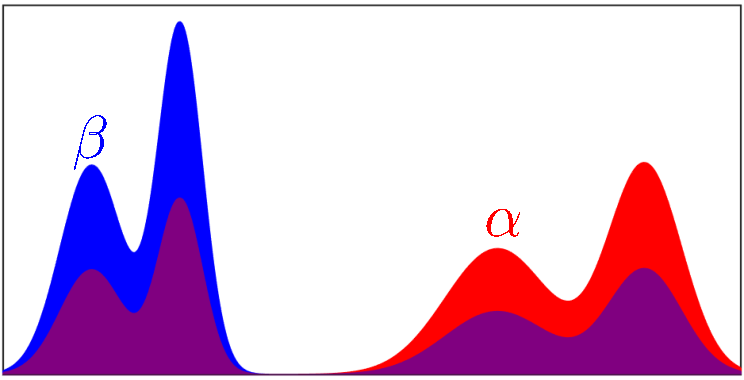
\includegraphics[width=.45\linewidth]{barycenters-1d/bary-eucl}  &
%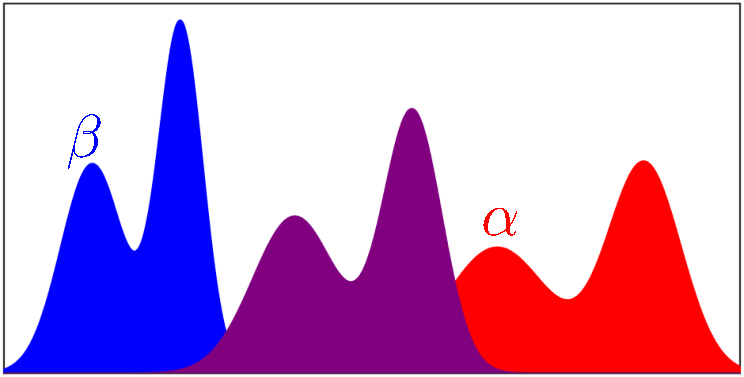
\includegraphics[width=.45\linewidth]{barycenters-1d/bary-ot} 
%\end{tabular}
%\caption{\label{fig-w-vs-eucl}
%Comparison of Wasserstein vs. Euclidean average. \todo{Blabla}
%}
%\end{figure}


%%%%%%%%%%%%%%%%%%%%%%%%%%%%%%%%%%
\section*{Notation}

\begin{itemize}
	\item $\range{n}$: set of integers $\{1,\dots,n\}$.
	\item $\ones_{n,m}$: matrix of $\RR^{n\times m}$ with all entries identically set to $1$. $\ones_{n}$: vector of ones.
	\item $\Identity_n$: identity matrix of size $n\times n$. 
	\item For $u\in\RR^n$, $\diag(u)$ is the $n\times n$ matrix with diagonal $u$ and zero otherwise.
	\item $\simplex_n$: probability simplex with $n$ bins, namely the set of probability vectors in $\RR^n_+$.	
	\item $(\a,\b)$:  histograms in the simplices $\simplex_n \times \simplex_m$. 
	\item $(\al,\be)$:  measures, defined on spaces $(\X,\Y)$.
	\item $\frac{\d\al}{\d\be}$: relative density of a measure $\al$ with respect to $\be$.
	\item $\density{\al} = \frac{\d\al}{\d x}$: density of a measure $\al$ with respect to Lebesgue measure.
	\item $(\al=\sum_i \a_i \delta_{x_i},\be=\sum_j \b_j \delta_{y_j})$: discrete measures supported on $x_1,\dots,x_n\in\X$ and $y_1,\dots,y_m\in\Y$.
	\item $\c(x,y)$: ground cost, with associated pairwise cost matrix $\C_{i,j}=(\c(x_i,y_j))_{i,j}$ evaluated on the support of $\al,\be$.
	\item $\pi$: coupling measure between $\al$ and $\be$, namely such that for any $A\subset\X, \pi(A\times \Y)= \al(A)$, and for any subset $B\subset \Y, \pi(\X\times B)= \be(B)$. For discrete measures $\pi = \sum_{i,j} \P_{i,j}\delta_{(x_i,y_j)}$.
	\item $\Couplings(\al,\be)$: set of coupling measures, for discrete measures $\CouplingsD(\a,\b)$.
	\item $\Potentials(\c)$: set of admissible dual potentials; for discrete measures $\PotentialsD(\C)$.
	\item $\T : \X \rightarrow \Y$: Monge map, typically such that $\T_\sharp \al = \be$.
	\item $(\al_t)_{t=0}^1$: dynamic measures, with $\al_{t=0}=\al_0$ and $\al_{t=1}=\al_1$.
	\item $\speed$: speed for Benamou--Brenier formulations; $\Moment=\al \speed$: momentum.
	\item $(\f,\g)$: dual potentials, for discrete measures $(\fD,\gD)$ are dual variables.
	\item $(\uD,\vD) \eqdef (e^{\fD/\varepsilon},e^{\gD/\varepsilon})$: Sinkhorn scalings.
	\item $\K \eqdef e^{-\C/\varepsilon}$: Gibbs kernel for Sinkhorn.
	% entropy
	\item $\flow$: flow for $\Wass_1$-like problem (optimization under divergence constraints).
	\item $\MKD_\C(\a,\b)$ and $\MK_\c(\al,\be)$: value of the optimization problem associated to the OT with cost $\C$ (histograms) and $\c$ (arbitrary measures).
	\item $\WassD_p(\a,\b)$ and $\Wass_p(\al,\be)$: $p$-Wasserstein distance associated to ground distance matrix $\distD$ (histograms) and distance $\dist$ (arbitrary measures).
	\item $\lambda\in\simplex_S$: weight vector used to compute the barycenters of $S$ measures.
	\item $\dotp{\cdot}{\cdot}$: for the usual Euclidean dot-product between vectors; for two matrices of the same size $A$ and $B$, $\dotp{A}{B} \eqdef \trace(A^\top B)$ is the Frobenius dot-product.
	\item $\f\oplus \g(x,y) \eqdef f(x)+g(y)$, for two functions $\f : \X \rightarrow \RR, \g : \Y \rightarrow \RR$, defines
		$\f \oplus \g : \X\times \Y \rightarrow \RR$.
	\item $\fD \oplus \gD \eqdef \fD \ones_m^\top + \ones_n \gD^\top \in \RR^{n\times m}$ for two vectors $\fD\in\RR^n$, $\gD\in\RR^m$.
	\item $\al \otimes \be$ is the product measure on $\X \times \Y$, \ie 
		$\int_{\X \times \Y} g(x,y) \d(\al\otimes\be)(x,y) \eqdef \int_{\X \times \Y} g(x,y) \d\al(x) \d\be(y)$.
	\item $\a \otimes \b \eqdef \a \b^\top \in \RR^{n \times m}$. 
	\item $\uD \odot \vD = (\uD_i \vD_i) \in \RR^n$ for $(\uD, \vD) \in (\RR^n)^2$.
\end{itemize}